\documentclass[a4paper, 12pt]{article}

%% Specify margins
\usepackage[margin=2cm]{geometry}

%% Use specific font
\usepackage{fontspec}
\setmainfont{Times New Roman}

\usepackage{mathtools}

%% ** Colors **
\usepackage{color} 
\usepackage[table]{xcolor}
\definecolor{linkcol}{RGB}{0,0,238}
\definecolor{lightgray}{gray}{0.8}

%% For hyperref (link for figures, equations and papers)
\usepackage{hyperref}
\hypersetup{
    breaklinks,
    baseurl       = http://,
    colorlinks    = true,
    linkcolor     = linkcol,
    citecolor     = linkcol,
    pdfborder     = 0 0 0
}

%% Bibliography
\usepackage{natbib}

%% Get label of figures bold
\usepackage[labelfont=bf]{caption}

% Write units properly
\usepackage{siunitx}
\DeclareSIUnit\year{yr}

\begin{document}
\renewcommand{\arraystretch}{1.5}

%TC:ignore
\section*{Summary}
%TC:endignore
\label{sec:Intro}
\section*{Introduction}

Scientific consensus has been reached for several years about the rapid environmental change we are experiencing, a rise of more than 0.8°C in the 1901-2012 period~\citep{stocker_ipcc_2013}. But, the high interannual variability makes temperature fluctuating around the increasing trend.

The increase of temperature caused several organisms to advance in their phenology, i.e. the timing of various seasons. There have been evidences of trend to precocity in plants in their flowering time and bud-burst date~\cite{alberto_adaptive_2011, gienapp_predicting_2013}.

Models generally take into account a single trait with a single optimal value maximizing the fitness of an individual~\citep{lande_quantitative_1982}. To mimic variable environments they either vary the optimum in a linear fashion or randomly fluctuate it around a given mean~\citep{lande_role_1996}.

As long-lived species trees experience selection differently from annual plants, they buffer selection across several years, because of their particular stage structure: seedlings and grown trees do not experience the same selection pressures~\citep{lande_quantitative_1982, coulson_dynamics_2008, barfield_evolution_2011, engen_evolution_2011}. 

Here we focused on the effect of fluctuations on a stage-structured tree population, with bud-burst date as the observed trait, and two different optima one from each stage.
We used a previously developed demographic and quantitative genetics models (see \ref{sec:M&M}), and implemented environmental fluctuations. Using \textsc{PHENOFIT}'s simulations we estimated those fluctuations in the wild.

\label{sec:M&M}
\section*{Materials and Methods}

\subsection*{Population model}

We used a previously developed model with stage-structure (Cite XXXXX Sandell et al.). We have two classes in our simulated tree population: immatures (I) and matures (M).
Explain the parameters.
The corresponding Lefkovitch matrix is:
\begin{equation}
	\label{eq:popmat}
	A =
	\begin{pmatrix}
	a_{II} & a_{IM} \\
	a_{MI} & a_{MM}
	\end{pmatrix}
	=
	\begin{pmatrix}
	s_{0} m f_{1} + s_{I} (1 - m) & s_{0} f_{2} \\
	s_{M} m & s_{M}
	\end{pmatrix}
\end{equation}

From the original model (Sandell et al. 2014) we implemented density-dependence, so that population will not continuously increase but reach a plateau (see Fig.~\ref{fig:dd}). We chose to implement density-dependence through seed germination and survival parameter $s_{0}$ using a Beverton-Holt function to avoid chaotic behaviors:
\begin{equation}
	\label{eq:ddfunc}
	s_{0} = \frac{s_{0, max}}{1 + k_{I} N_{I} + k_{M} N_{M}}
\end{equation}

with $k_{I}$ and $k_{M}$ the weights of immature ($N_{I}$) and mature ($N_{M}$) population respectively. $s_{0, max}$ is the maximum achievable $s_{0}$.

\subsection*{Life-history traits}

We considered certain life-history trait $s_{I}, f_{1}, f_{2}$ as gaussian for each individual such as:

\begin{equation}
	\label{eq:indlht}
	s_{I}(z) = s_{I}(\theta_{s})	\exp\left(-\frac{(z - \theta_{s})^2}{2\omega_{s}}\right)
\end{equation}

Averaging over the population it gives:

\begin{equation}
	\label{eq:poplht}
	\overline{s_{I}}(\overline{z_{I}}) = s_{I}(\theta_{s}) \sqrt{\frac{\omega_{s}}{\omega_{s}+P_{I}}}	\exp\left(-\frac{(\overline{z_{I}} - \theta_{s})^2}{2(\omega_{s}+P_{I})}\right)
\end{equation}

\subsection*{Iterations at each timestep}

Assuming the phenotype has a Gaussian distribution,  the mean genotypic value of matures and immatures at the next timestep is given by (\citealt{barfield_evolution_2011} Eq.5) :

\begin{equation}
	\begin{align}
		\label{eq:genotypic}
		\overline{g_{I}}' &= (c_{I M} \overline{g_{M}} + c_{I I} \overline{g_{I}}) 
			\left(c_{I M} G_{M} \frac{\partial \log \overline{a_{IM}}}{\partial \overline{z_{M}}} + c_{I I} G_{I} \frac{\partial \overline{a_{I I}}}{\partial \overline{z_{I}}} \\
		\overline{g_{M}}' &=	 (c_{M I} \overline{g_{I}} + c_{M M} \overline{g_{M}}) 
			\left(c_{M I} G_{I} \frac{\partial \log \overline{a_{M I}}}{\partial \overline{z_{I}}} + c_{M M} G_{M} \frac{\partial \overline{a_{M M}}}{\partial \overline{z_{M}}}
	\end{align}
\end{equation}

When there is a reproduction event, the phenotype of the newborn is computed as such:
...

\subsection*{Approximation under weak selection}

From \citep{engen_evolution_2011} and Sandell et al. we get the following approximation of the mean phenotype in the population:
\begin{equation}
	z = ...
\end{equation}

\subsection*{Fluctuating environment}

To mimic a fluctuating environment, the optimums are fluctuating in various ways around a mean.

Under fluctuations we get another approximation supposing weak selection \citep{engen_evolution_2011}:
...

\subsection*{Trend in change}
...

\subsection*{Phenofit data}

PHENOFIT is phenology model...

On 6 localities (see map .) we had modelled budburst date and predicted fitnesses $\pm$ 21 days around this date, from these data we predicted the optimums fluctuations:
...
All statistical analysis were made using R, for the plots we used the package ggplot2.

\begin{table}
\begin{center}
	\rowcolors{1}{white}{lightgray}
	\begin{tabular}{l c c}
		\hline \hline
		Parameter & Notation & Value \\
		\hline
		\multicolumn{3}{l}{\textbf{Life Cycle}} \\
		Optimal phenotype for fecundity & $\theta_{f}$ & 100 \\
		Optimal phenotype for immature survival & $\theta_{s}$ & 130 \\
		Fecundity function width & $\omega_{f}$ & 400 \\
		Survival function width & $\omega_{s}$ & 400 \\
		Heritability & $h^2$ & 0.5 \\
		Phenotypic variance of immatures & $P_{I}$ & 40 \\
		Phenotypic variance of matures & $P_{M}$ & 40 \\
		Genotypic variance of immatures & $G_{I} = P_{I} \times h^2$ & 20 \\
		Genotypic variance of matures & $G_{M}$ & 20 \\
		Survival of immature at phenotypic optimum & $\overline{s_{I}}(\overline{z} = \theta_{s})$ & 0.8 \\
		Fecundity of first time reproducers at optimum & $\overline{f_{1}}(\overline{z} = \theta_{f})$ & 100 \\
		Fecundity of experienced reproducers at optimum & $\overline{f_{2}}(\overline{z} = \theta_{f})$ & 200 \\
		Maturation rate of immature & $m$ & 0.02 \\
		Combined survival and germination rate of seed & $s_{0}$ & 0.03 \\
		Survival of mature stage & $s_{M}$ & 0.99 \\
		\multicolumn{3}{l}{\textbf{Density-dependence}} \\
		Maximum $s_{0}$ in density-dependence function & $s_{0, max}$ & 0.12 \\
		Decreasing factor due to immatures & $k_{I}$ & 0.0001 \\
		Decreasing factor due to matures & $k_{M}$ & 0.005 \\
		\multicolumn{3}{l}{\textbf{Fluctuations}} \\
		Sensitivity of optimum for fecundity to fluctuation & $\alpha_{f}$ & 5 \\
		Sensitivity of optimum for survival to fluctuation & $\alpha_{s}$ & 5 \\
		Noise variance for fecundity & $\sigma_{\xi_{f}}^2$ & 3.725 \\
		Noise variance for survival & $\sigma_{\xi_{s}}^2$ & 3.725 \\
		Correlation between noises & $\rho_{N}$ & 0.5 \\
		\hline \hline
	\end{tabular}
	\caption{Standard parameter set}
	\label{tab:params}
\end{center}
\end{table}

%Basic explanation of the models. We modeled a stage-structured population in two stages: immatures and matures. The demography is given by a transition matrix, with...
%
%\subsection*{Under constant environment, no plasticity}
%
%Using \citet{lande_adaptation_2009}, under weak selection we have:
%\begin{equation}
%	\label{eq:dz}
%	\Delta\overline{z} = \frac{d\ln\overline{\lambda}(\overline{z})}{d\overline{z}} = \frac{1}{\overline{\lambda}(\overline{z})} \frac{d\overline{\lambda}(\overline{z})}{d\overline{z}}
%\end{equation}
%
%And we have:
%\begin{align*}
%	\overline{\lambda}(\overline{z}) &= \sum_{i,j}{v_{i} u_{j} \overline{a_{ij}}} \\
%	&= v_{I} u_{I} \overline{a_{II}} + v_{I} u_{M} \overline{a_{IM}} + v_{M} u_{I} \overline{a_{MI}} + v_{M} u_{M} \overline{a_{MM}}
%\end{align*}
%
%With $\overline{a_{ij}}$ the expected values of the coefficent of the transition matrix. Thus,
%\begin{align}
%	\overline{\lambda}(\overline{z}) &= v_{I} u_{I} \left[ \overline{f_{1}}(\overline{z}) m s_{0} + (1-m) \overline{s_{I}}(\overline{z}) \right] + v_{I} u_{M} s_{0} \overline{f_{2}}(\overline{z}) \nonumber \\
%	&\quad + v_{M} u_{I} m s_{M} + v_{M} u_{M} s_M \\
%	\label{eq:dlambda}
%	\frac{d\overline{\lambda}(\overline{z})}{d\overline{z}} &= v_{I} u_{I} \left[ \frac{d\overline{f_{1}}(\overline{z})}{d\overline{z}} m s_{0} + (1-m) \frac{d\overline{s_{I}}(\overline{z})}{d\overline{z}} \right] + v_{I} u_{M} s_{0} \frac{d\overline{f_{2}}(\overline{z})}{d\overline{z}}
%\end{align}
%
%Because $f_{i}$ and $s_{I}$ are gaussians we can write the population means $\overline{f_{i}}$ and $\overline{s_{I}}$ easily.
%
%\begin{subequations}
%	\begin{align}
%	\label{eq:meanf}
%		\overline{f_{1}}(\overline{z}) &= f_{1}(\theta_{f}) \sqrt{\frac{\omega_{f}}{\omega_{f} + P_{I}}} \exp\left(-\frac{(\overline{z}-\theta_{f})^2}{2(\omega_{f}+P_{I})}\right) \\
%		\overline{f_{2}}(\overline{z}) &= f_{2}(\theta_{f}) \sqrt{\frac{\omega_{f}}{\omega_{f} + P_{M}}} \exp\left(-\frac{(\overline{z}-\theta_{f})^2}{2(\omega_{f}+P_{M})}\right) \\
%		\overline{s_{I}}(\overline{z}) &= s_{I}(\theta_{s}) \sqrt{\frac{\omega_{s}}{\omega_{s} + P_{I}}} \exp\left(-\frac{(\overline{z}-\theta_{s})^2}{2(\omega_{s}+P_{I})}\right)
%	\end{align}
%\end{subequations}
%
%Thus we can derive these expression with respect to $\overline{z}$:
%
%\begin{align}
%	\label{eq:dfdz}
%	\frac{\partial \overline{f_{1}}(\overline{z}) }{ \partial \overline{z} } &= f_{1}(\theta_{f}) \sqrt{\frac{\omega_{f}}{\omega_{f} + P_{I}}} \frac{\partial \exp \left(-\frac{(\overline{z}-\theta_{f})^2}{2(\omega_{f}+P_{I})}\right)}{\partial\overline{z}} \nonumber \\
%	&= f_{1}(\theta_{f}) \sqrt{ \frac{\omega_{f}}{ \omega_{f} + P_{I}}}\exp\left(-\frac{(\overline{z}-\theta_{f})^2}{2(\omega_{f}+P_{I})}\right) \frac{\theta_{f} - \overline{z}}{\omega_{f} + P_{I}} \nonumber \\
%	&= \overline{f_{1}}(\overline{z}) \frac{\theta_{f} - \overline{z}}{\omega_{f} + P_{I}}
%\end{align}
%
%We obtain similar formulas for $\overline{f_{2}}$ and $\overline{s_{I}}$. Plugging \eqref{eq:dfdz} into \eqref{eq:dlambda} we have:
%
%\begin{equation}
%	\label{eq:finaldlambda}
%	\frac{d\overline{\lambda}(\overline{z})}{d\overline{z}} = v_{I} u_{I} \left[ \frac{\theta_{f} - \overline{z}}{\omega_{f} + P_{I}} m s_{0} + (1-m) \frac{\theta_{s} - \overline{z}}{\omega_{s} + P_{I}} \right] + v_{I} u_{M} s_{0} \frac{\theta_{f} - \overline{z} }{\omega_{f} + P_{M}}
%\end{equation}
%
%Using \eqref{eq:finaldlambda} into \eqref{eq:dz} gives us after rearranging:
%We have for variations of phenotype, under weak selection:
%\begin{equation}
%	\label{eq:cstdeltaz}
%	\Delta\overline{z} = 
%		(\theta_{f} - \overline{z})
%		\left[ \frac{ v_{I} u_{I} G_{I} s_{0} m \overline{f_{1}} }{ \lambda (P_{I}+\omega_{f}) }
%			+ \frac{ v_{I} u_{M} G_{M} s_{0} \overline{f_{2}} }{ \lambda (P_{M} + \omega_{f}) }
%		\right]
%		+ (\theta_{s} - \overline{z})
%		\left[ \frac{ v_{I} u_{I} G_{I} \overline{s_{I}} (1-m) }{ \lambda (P_{I}+\omega_{s}) }
%		\right]
%\end{equation}
%
%Within the square brackets, we see weighting average of fecundity and survival. Thus, we define them as $\gamma_{f}$ and $\gamma_{s}$ such as:
%
%\begin{subequations}
%	\begin{equation}
%	\label{eq:gammaf}
%	\gamma_{f} = \frac{v_{I} u_{I} s_{0} m \overline{f_{1}} }{\lambda(P_{I}+\omega_{f})} + \frac{ v_{I} u_{M} \frac{G_{M}}{G_{I}} s_{0} \overline{f_{2}}}{\lambda ( P_{M} + \omega_{f} )}
%	\end{equation}
%	and
%	\begin{equation}
%	\label{eq:gammas}
%	\gamma_{s} = \frac{ v_{I} u_{I} \overline{s_{I}} (1-m) }{\lambda(P_{I}+\omega_{s})}
%	\end{equation}
%\end{subequations}
%
%We end up having a simpler expression for $\Delta\overline{z}$ under constant environment:
%
%\begin{align}
%	\Delta\overline{z} &= -G_{I} \left[ \gamma_{f}(\overline{z} - \theta_{f}) + \gamma_{s}(\overline{z} - \theta_{s}) \right] \nonumber \\
%	\Delta\overline{z} &= - G_{I} \gamma(\overline{z} - \theta_{v})
%\end{align}
%
%with
%\begin{align}
%	\label{eq:gamma}
%	\gamma &= \gamma_{f} + \gamma_{s} \\
%	\label{eq:thetav}
%	\theta_{v} &= \frac{\frac{\gamma_{f}}{\gamma_{s}}\theta_{f} + \theta_{s}}{\frac{\gamma_{f}}{\gamma_{s}} + 1}
%\end{align}
%
%\subsection*{Under varying environment, without plasticity}
%From \citet{engen_evolution_2011}, we derived equations for mean variation of phenotype on our model.
%
%We supposed an auto-correlated fluctuating environment $\epsilon_{t}$ influencing optimums $\theta_{i}$ such as:
%\begin{align}
%	\label{eq:epstheta}
%\left\{
%	\begin{aligned}
%		\theta_{i}(t) &= \overline{\theta}_{i} + \alpha_{i}\epsilon_{t}\\
%		\epsilon_{t+1} &= (1-\rho)\overline{\epsilon} + \rho\epsilon_{t} + \xi
%	\end{aligned}
%\right.
%\end{align}
%with $\alpha_{i}$ the dependence factor of the optimum on the environment, $\rho$ the auto-correlation coefficient of the environment, $\overline{\epsilon}$ the expected environment and $\xi$ a gaussian noise vector with variance $\sigma^{2}_{\xi}$ and mean $0$. We chose $\overline{\epsilon}=0$ to simplify the calculations so that $\epsilon_{t+1} = \rho\epsilon_{t} + \xi$, we can see that:
%
%\begin{align}
%	\theta_{i}(t+1) &= \overline{\theta}_{i} + \alpha_{i}\epsilon_{t+1} \nonumber \\
%	&= \overline{\theta}_{i} + \alpha_{i}(\rho\epsilon_{t} + \xi) \nonumber \\
%	&= \overline{\theta}_{i} + \alpha_{i}\rho(\frac{\theta_{i}(t)-\overline{\theta}_{i}}{\alpha_{i}}) + \alpha_{i}\xi \nonumber \\
%	\label{eq:thetait}
%	\theta_{i}(t+1) &= \overline{\theta}_{i}(1-\rho) + \rho\theta_{i}(t) + \alpha_{i}\xi
%\end{align}
%
%The auto-correlation in the environment $\epsilon_{t}$ causes $\theta_{i}$ to be auto-correlated with the same correlation coefficient $\rho$.
%
%Using the same approach as in a constant environment, under weak selection, we end up having a similar equation than \eqref{eq:cstdeltaz} but with optimum depending on environment:
%
%\begin{equation}
%	\label{eq:deltazt}
%	\Delta\overline{z}_{t} = 
%		(\theta_{f}(t) - \overline{z_{t}})
%		\left[ \frac{ v_{I} u_{I} G_{I} s_{0} m \overline{f_{1}} }{ \lambda_{t} (P_{I}+\omega_{f}) }
%			+ \frac{ v_{I} u_{M} G_{M} s_{0} \overline{f_{2}} }{ \lambda_{t} (P_{M} + \omega_{f}) }
%		\right]
%		+ (\theta_{s}(t) - \overline{z_{t}})
%		\left[ \frac{ v_{I} u_{I} G_{I} \overline{s_{I}} (1-m) }{ \lambda_{t} (P_{I}+\omega_{s}) }
%		\right]
%\end{equation}
%
%Plugging \eqref{eq:epstheta} in \eqref{eq:deltazt} we obtain
%
%\begin{subequations}
%	\begin{align}
%		\Delta\overline{z}_{t} &= 
%			(\overline{\theta}_{f} + \alpha_{f}\epsilon_{t} - \overline{z_{t}})
%			\left[ \frac{ v_{I} u_{I} G_{I} s_{0} m \overline{f_{1}} }{ \lambda_{t} (P_{I}+\omega_{f}) }
%				+ \frac{ v_{I} u_{M} G_{M} s_{0} \overline{f_{2}} }{ \lambda_{t} (P_{M} + \omega_{f}) }
%			\right]
%			+ (\overline{\theta}_{s} + \alpha_{s}\epsilon_{t} - \overline{z_{t}})
%			\left[ \frac{ v_{I} u_{I} G_{I} \overline{s_{I}} (1-m) }{ \lambda_{t} (P_{I}+\omega_{s}) }
%			\right] \nonumber \\
%	\end{align}
%	Defining the same $\gamma_{f}$, $\gamma_{s}$ and $\theta_{v}$ as in \eqref{eq:gammaf}, \eqref{eq:gammas} and \eqref{eq:thetav}, respectively:
%	\begin{align}
%			\Delta\overline{z}_{t} &= G_{I} \left[(\overline{\theta}_{f} + \alpha_{f}\epsilon_{t} - \overline{z_{t}})
%			\gamma_{f}
%			+ (\overline{\theta}_{s} + \alpha_{s}\epsilon_{t} - \overline{z_{t}})
%			\gamma_{s} \right] \nonumber \\
%			&= - G_{I} \left[ \gamma_{f}(\overline{z_{t}} - \theta_{f}) + \gamma_{s}(\overline{z_{t}} - \theta_{s}) \right] -G_{I} \epsilon_{t} \left( \gamma_{f}\alpha_{f} + \gamma_{s}\alpha_{s} \right) \nonumber \\
%			\label{eq:deltaztdeltaz}
%			\Delta\overline{z}_{t} &= \Delta\overline{z} + G_{I} \epsilon_{t} \left( \gamma_{f}\alpha_{f} + \gamma_{s}\alpha_{s} \right) \\
%			&= -G_{I}\gamma(\overline{z_{t}} - \theta_{v})  + G_{I} \epsilon_{t} \left( \gamma_{f}\alpha_{f} + \gamma_{s}\alpha_{s} \right) \nonumber \\
%			&= -G_{I}\gamma \left(\overline{z_{t}} - \theta_{v} - \epsilon_{t} \frac{\gamma_{f}\alpha_{f}+\gamma_{s}\alpha_{s}}{\gamma} \right) \nonumber \\
%			\label{eq:totaldeltazt}
%			\Delta\overline{z}_{t} &= -G_{I}\gamma (\overline{z_{t}} - \theta_{v} - \alpha_{v}\epsilon_{t})
%	\end{align}
%\end{subequations}
%With $\alpha_{v}$ a weighted component between $\alpha_{f}$ and $\alpha_{s}$, defined in similar fashion as $\theta_{v}$ in \eqref{eq:thetav}:
%\begin{align}
%	\alpha_{v} &= \frac{\gamma_{f}\alpha_{f}+\gamma_{s}\alpha_{s}}{\gamma} \nonumber \\
%	&= \frac{ \gamma_{f}\alpha_{f}+\gamma_{s}\alpha_{s} }{\gamma_{f}+\gamma_{s}} \nonumber \\
%	\alpha_{v} &=\frac{\frac{\gamma_{f}}{\gamma_{s}}\alpha_{f}+\alpha_{s}}{ \frac{\gamma_{f}}{\gamma_{s}} + 1}
%\end{align}
%
%\subsubsection*{Estimating variance of $\overline{z}_{t}$}
%
%Taking \eqref{eq:totaldeltazt} we can estimate variance of $\overline{z}_{t}$. Using the same process as \citet{engen_evolution_2011}. Indeed, \eqref{eq:totaldeltazt} has the form:
%\begin{equation}
%	\label{eq:defdeltaat}
%	\Delta A_{t}=-D A_{t} + e_{t}
%\end{equation}
% with $A_{t}=\overline{z_{t}} - \theta_{v}$, $D = G_{I} \gamma$ and $e_{t} = D\alpha_{v}\epsilon_{t}$. \eqref{eq:defdeltaat} has a stationary solution:
%
%\begin{subequations}
%	\begin{equation}
%		\label{at+1}
%		A_{t+1} = (1-D)^{t+1} A_{0} + \sum_{r=0}^{t} (1-D)^{r} e_{t-r}
%	\end{equation}
%	
%	If we consider the evolution of $A_{t}$ over a long time, \eqref{at+1} becomes, because $(1-D) < 1$:
%	
%	\begin{align}
%		\label{atsum}
%		A_{t} = \sum_{r=0}^{\infty}e_{t-r}(1-D)^{r}
%	\end{align}
%\end{subequations}
%
%We want to estimate how will $\overline{z}_{t}$ move away from the mean because of environmental fluctuations, that is why we compute its variance. From \eqref{at+1}:
%\begin{equation}
%	\begin{aligned}
%	\text{Var}(A_{t}) &= \text{Var} \left[ \sum_{r=0}^{\infty}e_{t-r}(1-D)^{r} \right] \\
%	&= \sum_{r=0}^{\infty} \text{Var} \left[ e_{t-r}(1-D)^{r} \right] \\
%	&=  \sum_{r=0}^{\infty} \text{Var} \left[ \epsilon_{t-r} D \alpha_{v} (1-D)^{r} \right] \\
%	&\overset{\text{def}}{=} \sigma_{\epsilon}^{2} D^{2} \alpha_{v}^{2} \sum_{r=0}^{\infty} (1-D)^{2r} \\
%	\text{Var}(A_{t}) &= \sigma_{\epsilon}^{2} D^{2} \alpha_{v}^{2} \frac{1}{1-(1-D)^{2}} \\
%	\text{Var}(\overline{z_{t}}) &\overset{\text{def}}{=} \sigma_{\epsilon}^{2} G_{I}^{2}\gamma^{2} \alpha_{v}^{2} \frac{1}{G_{I}\gamma(2-G_{I}\gamma)} \\
%	\label{eq:varzws}
%	\text{Var}(\overline{z_{t}}) &\overset{\gamma \to 0}{=} \frac{1}{2} G_{I}\gamma\sigma_{\epsilon}^{2}\alpha_{v}^{2}
%	\end{aligned}
%\end{equation}

\label{sec:Res}
\section*{Results}

\subsection*{Constant environment and density-dependence}

We used the previously developed model in \citetext{Sandell et al. 2014, master's thesis} and simulated (see~\autoref{fig:dd}) a tree population for 150 years in constant environment, with and without density-dependence on $s_0$, to model a more realistic demography.

Indeed, density-dependence introduced a limit in the population (\autoref{fig:dd} right panel), as the number of mature and immature individuals seem to converge respectively to $18000$ and $10000$ individuals, while without density-dependence the population is exponentially growing.

Looking at the phenotype, we started from exactly the same starting point $z=116$ for phenotypic and genotypic values. Without density-dependence, the population quickly converge to the equilibrium phenotype ($\overline{z_{weak}}$ given by the approximation in~\autoref{eq:zweak}), $\overline{z_{weak}} = 166$ in this case. With density-dependence the equilibrium is shifted upward ($\overline{z_{weak, dd}} = 121.8$).

This shift is due to the decrease of $s_0$ in the density-dependent model, indeed because of the initial population $s_{0, dd} = 1.18 10^-3$ while $s_0 = 0.03$ without density-dependence. This difference, all else being equal, changes the equilibrium of $\overline{z_{weak}}$. With a lower seed survival, the equilibrium is shifted towards $\theta_s$, i.e. the survival optimum for immature, because it compensates to maintain the demographic equilibrium (growth rate = 1).

Within the density-dependent model the mean immature phenotype $\overline{z_I}$ converge quicker than the mean mature phenotype $\overline{z_M}$ to the equilibrium. It is because of stage-structured nature of our model, the mature stage is a combination of individuals that lived for around 40 generations (given our life-cycle), it buffers adaptation. To change $\overline{z_M}$, the individual have first to be closer to $\overline{z_{weak}}$ than to survive for a certain number of years and become mature. While the newborns of the given generation are already closer to the equilibrium.

\begin{figure}[ht!]
	\centering
	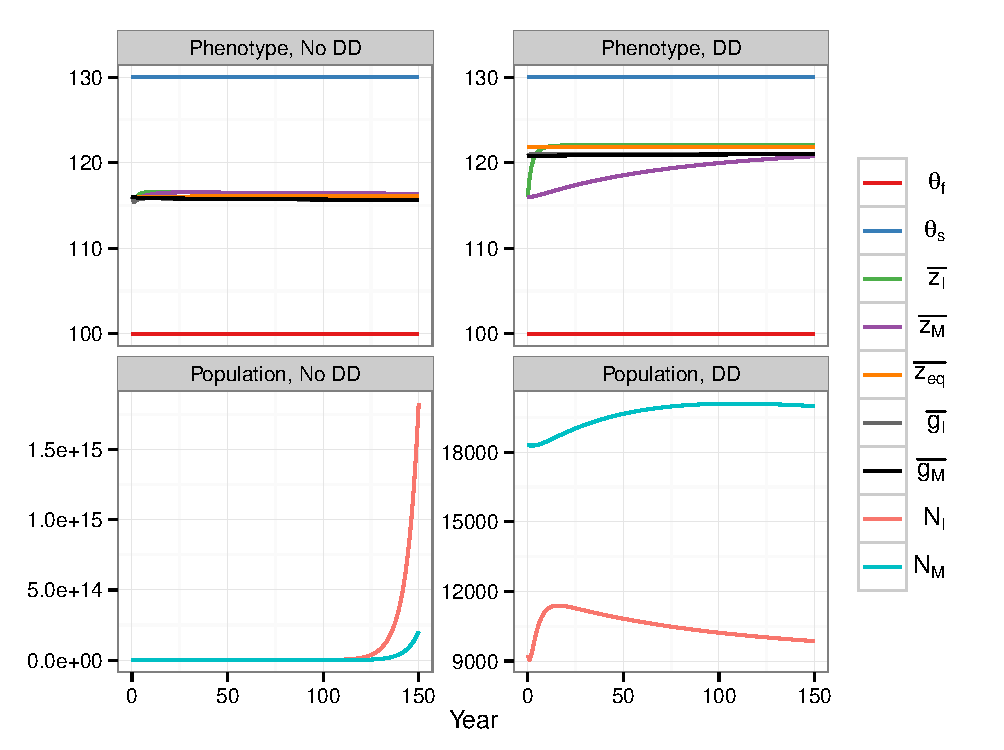
\includegraphics[scale=1]{Figures/DDphenopop.pdf}
	\caption{\textbf{Effect of density-dependence on phenotypes and populations}. \textbf{Left panel}: Phenotype variations in population ($\overline{z_I}, \overline{z_M}$) with their corresponding genotypic values ($\overline{g_I}, \overline{g_M}$) all starting from $z = 166$, and the approximation given by \autoref{eq:zweak}; \textbf{right panel}: demography, number of immature individuals ($N_I$, red), number of mature individuals ($N_M$, blue). Starting from Stable-Stage Distribution (SSD) in constant environment, note the logarithmic scale used.}
	\label{fig:dd}
\end{figure}

\subsection*{Fluctuating optimums}

To mimic a more realistic environment we made the optimums fluctuate, with various correlations between them. We simulated three populations using the same random seed. We only vary correlations between noises.

Explain in the text correlation of $z_{I}$ with $\theta_{s}(t)$

\begin{figure}[ht!]
	\centering
	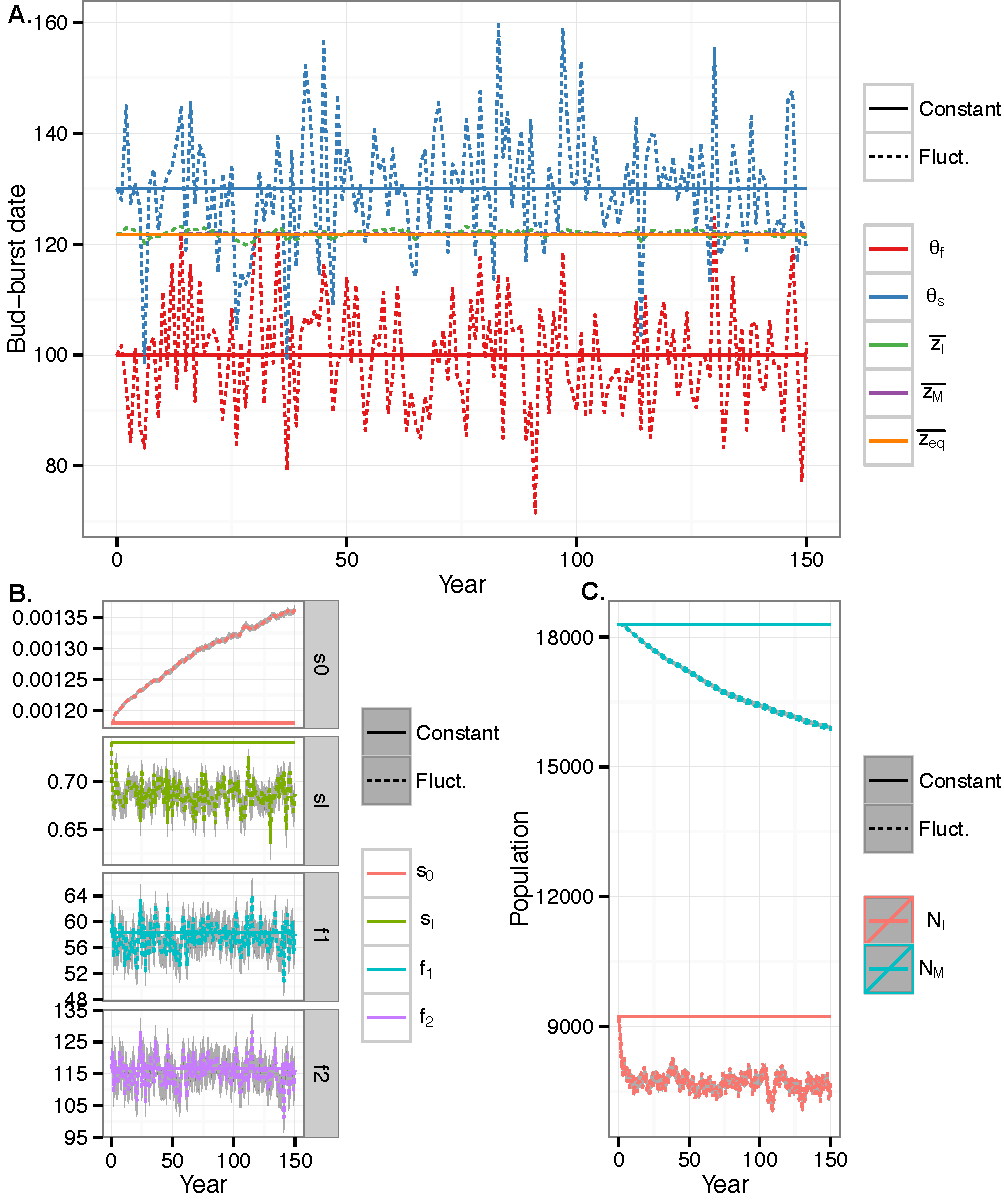
\includegraphics[scale=1]{Figures/PhenoLHTwithCorr.pdf}
	\caption{\textbf{Effect of the correlation of fluctuations on phenotypes and life-history traits}. Correlation coefficient $\rho_{N}$ values of noises are indicated at the the top of each column. Phenotype and approximations are shown in julian days, $\overline{z_\epsilon}$ is the approximation from \autoref{eq:zfluct}. Mean fecundities are in number of seeds produced. The two bottom rows are survival rates, the top one is $\overline{s_I}$ the mean survival of immature individuals, the bottom one is $s_0$ the rate of survival and germination of seeds (see~\nameref{sec:M&M}).}
	\label{fig:corr}
\end{figure}

\subsection*{Trend in the environment}

\begin{figure}[ht!]
	\centering
	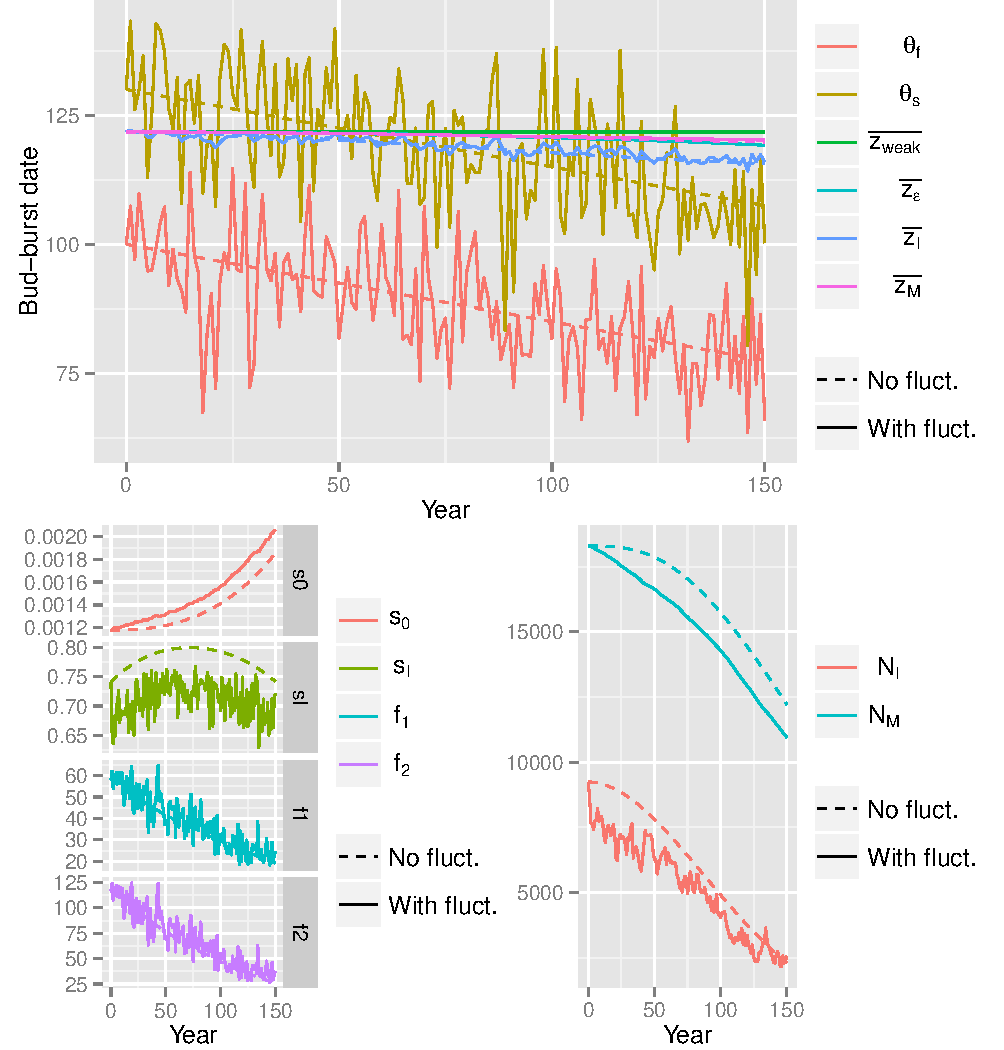
\includegraphics[scale=1]{Figures/Trend.pdf}
	\caption{\textbf{Mixed influences of trend and fluctuations on the population}. \textbf{Top panel}: Phenotype evolution with and without fluctuations; \textbf{Bottom:} (\textbf{Left}) Life-History Traits evolution depending on fluctuations, (\textbf{Right}) demography.}
	\label{fig:thetaf}
\end{figure}

Decreasing optimums through time to mimic the advance in phenology with climate change.

\textbf{Figure:} Trend 2 panels with and without fluctuations, simulations results phenotype/time (with and without DD)

\subsection*{Estimation of the fluctuations}

\begin{figure}[ht!]
	\centering
	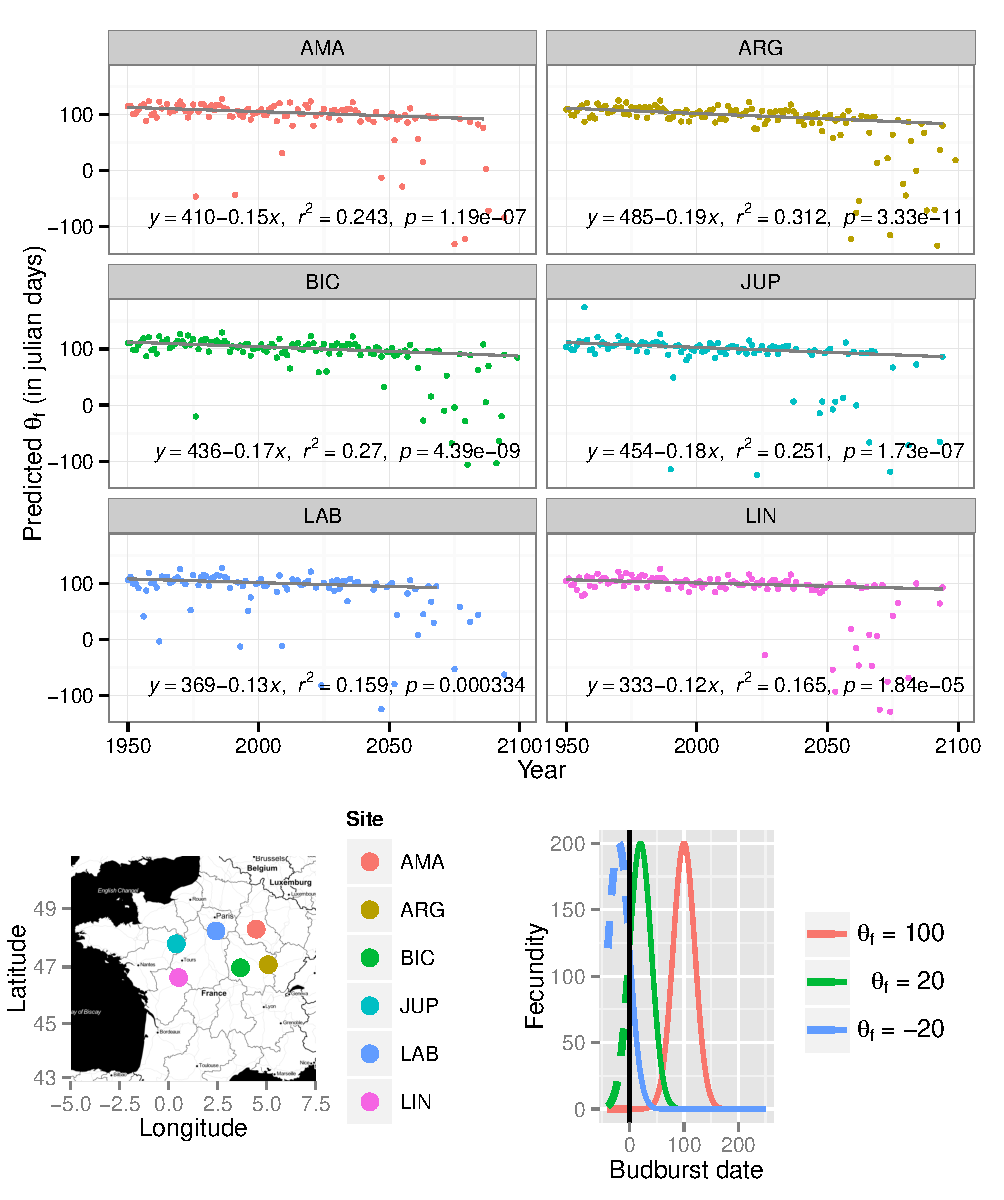
\includegraphics[scale=1]{Figures/optsmaps.pdf}
	\caption{\textbf{$\theta_{f}$ estimations from PHENOFIT data}. Top 3 rows: estimations of $\theta_f$ for each study site see \nameref{sec:M&M} for details. Bottom left panel: map of the study sites. Bottom right panel: Theoretical fecundity functions with parameters from~\autoref{tab:params} with values of $\theta_f$ equals to $100$, $20$ and $-20$, solid lines indicate achievable phenotype, dashed lines show theoretical curves but unreachable phenotypes.}
	\label{fig:thetaf}
\end{figure}

From 6 localities (map \autoref{fig:thetaf} bottom left) of \textsc{PHENOFIT} data, we computed $\theta_f$ values at these locations (top 3 rows of \autoref{fig:thetaf}). For the 6 sites, predicted $\theta_f$ decrease with time, it is more precocious as time passes. This observation matches the advance of phenology observed in the literature because of climate change.

Over the general trend, we observe a small amplitude variation around 20 days, corresponding to year to year change in $\theta_f$ and some dramatic decreases in its values, sometimes reaching negative values (For example at BIC site in 1976). The frequency of these events increase with time as they become \"normal\" after 2050 for all sites. Note that those event are biased towards the decrease of $\theta_f$, as there is no equivalent dramatic increases.

The negative values of $\theta_f$ computed in \autoref{fig:thetaf}, may seem striking as there is no such thing as a negative bud-burst date! However, as bottom right panel of \autoref{fig:thetaf} shows, we can have negative value of $\theta_f$ and still have achievable phenotypes. And if $\theta_f$ is very negative for a given year (less than -100 in 2048 for LAB), it means that will be no reproduction this year.

We excluded those extreme events to estimate the trend in the variation of $\theta_f$ (see~\nameref{sec:M&M}). Using linear regression on $\theta_f$ with time, we found a rate of \SI{-0.15}{\day\per\year}, with normal residuals having a variance of \SI{93.1}{\day\squared} (data not shown, $R^2=0.2435$, $p=1.185 10^{-7}$, $F=32.5$ with $101$ d.f.).

We investigated to know if there was a break between years modeled from real data by \textsc{PHENOFIT} (before 2001) and years modeled using climate models with climate change included (from 2001). We performed the same regression as above, without taking apart the extreme values, for all sites, splitting the data before 2001 and from 2001. Taking all years, for each site.

\label{sec:Disc}
\section*{Discussion}

We modeled a stage-structured tree population using a quantitative genetics approach, with bud-burst date varying between two optima. We predicted phenotype evolution in the next 150 years. Using \textsc{PHENOFIT} simulation results we computed values for one of the optima. According to simulations, an increasing number of extreme events will happen in the next century where all fecundities will be equal to zero.

As expected in the literature, we found a decreasing trend in the variation of optima, i.e. a trend to precocity of phenology \citep{aitken_adaptation_2008, ehrlen_timing_2009}. Because of the general increase in temperature, organisms advance their phenology to track their original environment, either by genetic change or plasticity~(\citealt{savolainen_genetic_2004}, reviewed in \citealt{merila_climate_2014}).

Increasing evidences underline the role of plasticity in adaptation to changes.

Genotypic ($\overline{g_i}$) and phenotypic ($\overline{z_i}$) values are different in our simulations (see~\autoref{fig:dd}); because of both stage-structure and the two optima we use.


With trend (\autoref{fig:trend}), counter-intuitively, there is no difference of in adaptation speed with and without fluctuations. We could have expected an additional cost of fluctuations: if the population would have tracked fluctuations closely, then a increased noise variance would have decrease fitness dramatically. Since it is not the case for reasons cited above, we see no cost of fluctuations when there is a general trend in the environment.

The mean phenotype in immature individuals $\overline{z_I}$ changes faster than the mean phenotype in mature individuals $\overline{z_M}$, there is a difference of adaptation speed between stages. The stage-structure of our population explains the different behaviors among the two classes. 

Our model was parametrized according to the sessile oak life-cycle (\textit{Quercus petraea} spp.) — using the \textsc{PHENOFIT} simulations to predict fluctuations and trend in the optima — the species does not go extinct in the next 150 years (\autoref{fig:trend}). Climate change has still dramatic demographic consequences, the population halving in less than 100 years. The sessile oak would be left more vulnerable demographically as it increases genetic drift and the potential consequences of dramatic events.

Those estimations and fluctuations do not include the extreme years when all fecundities are equal to zero, i.e. the selection gradient is zero, which should affect adaptation dynamics. Modeling correctly the variations of optima values would lead to more realistic behavior, it could be done by drawing the optima from an almost Gaussian distribution with a very long tail towards negative values.

Phenotypic plasticity should also be taken into account in a future model as it slows down genetic adaption. It has been shown to be an important component of adaptation to environmental changes~\citep{aitken_adaptation_2008}.

%TC:ignore
%\label{sec:Ack}
\section*{Authors Contributions and Acknowledgments}

M. Grenié did the analyses and simulations, based on L. Sandell's work. O. Ronce and LM. Chevin supervised the project. A. Duputié shared \textsc{PHENOFIT} outputs. I. Chuine advised the project about \textsc{PHENOFIT} outputs.

I would like to thank Ophélie Ronce for being an extremely patient supervisor, Luis-Miguel Chevin and Isabelle Chuine for the discussions we had about the project. I thank Guillaume Martin for being an awesome office-mate. Finally, I would like to thank the whole "Metapopulations" team at ISEM for their welcome.
%TC:endignore

\section*{References}
\bibliographystyle{cell.bst}
\bibliography{Bibliography}

\begin{table}
\begin{center}
	\rowcolors{1}{white}{lightgray}
	\begin{tabular}{l c c}
		\hline \hline
		Parameter & Notation & Value \\
		\hline
		\multicolumn{3}{l}{\textbf{Life Cycle}} \\
		Optimal phenotype for fecundity & $\theta_{f}$ & 100 \\
		Optimal phenotype for immature survival & $\theta_{s}$ & 130 \\
		Fecundity function width & $\omega_{f}$ & 400 \\
		Survival function width & $\omega_{s}$ & 400 \\
		Heritability & $h^2$ & 0.5 \\
		Phenotypic variance of immatures & $P_{I}$ & 40 \\
		Phenotypic variance of matures & $P_{M}$ & 40 \\
		Genotypic variance of immatures & $G_{I} = P_{I} \times h^2$ & 20 \\
		Genotypic variance of matures & $G_{M}$ & 20 \\
		Survival of immature at phenotypic optimum & $\overline{s_{I}}(\overline{z} = \theta_{s})$ & 0.8 \\
		Fecundity of first time reproducers at optimum & $\overline{f_{1}}(\overline{z} = \theta_{f})$ & 100 \\
		Fecundity of experienced reproducers at optimum & $\overline{f_{2}}(\overline{z} = \theta_{f})$ & 200 \\
		Maturation rate of immature & $m$ & 0.02 \\
		Combined survival and germination rate of seed & $s_{0}$ & 0.03 \\
		Survival of mature stage & $s_{M}$ & 0.99 \\
		\multicolumn{3}{l}{\textbf{Density-dependence}} \\
		Maximum $s_{0}$ in density-dependence function & $s_{0, max}$ & 0.12 \\
		Decreasing factor due to immatures & $k_{I}$ & 0.001 \\
		Decreasing factor due to matures & $k_{M}$ & 0.005 \\
		\multicolumn{3}{l}{\textbf{Fluctuations}} \\
		Sensitivity of optimum for fecundity to fluctuation & $\alpha_{f}$ & 5 \\
		Sensitivity of optimum for survival to fluctuation & $\alpha_{s}$ & 5 \\
		Noise variance for fecundity & $\sigma_{\xi_{f}}^2$ & 3.725 \\
		Noise variance for survival & $\sigma_{\xi_{s}}^2$ & 3.725 \\
		Correlation between noises & $\rho_{N}$ & 0.5 \\
		Trend coefficient & $k$ & -0.15 \\
		\hline \hline
	\end{tabular}
	\caption{Standard parameter set}
	\label{tab:params}
\end{center}
\end{table}

\begin{figure}[ht!]
	\centering
	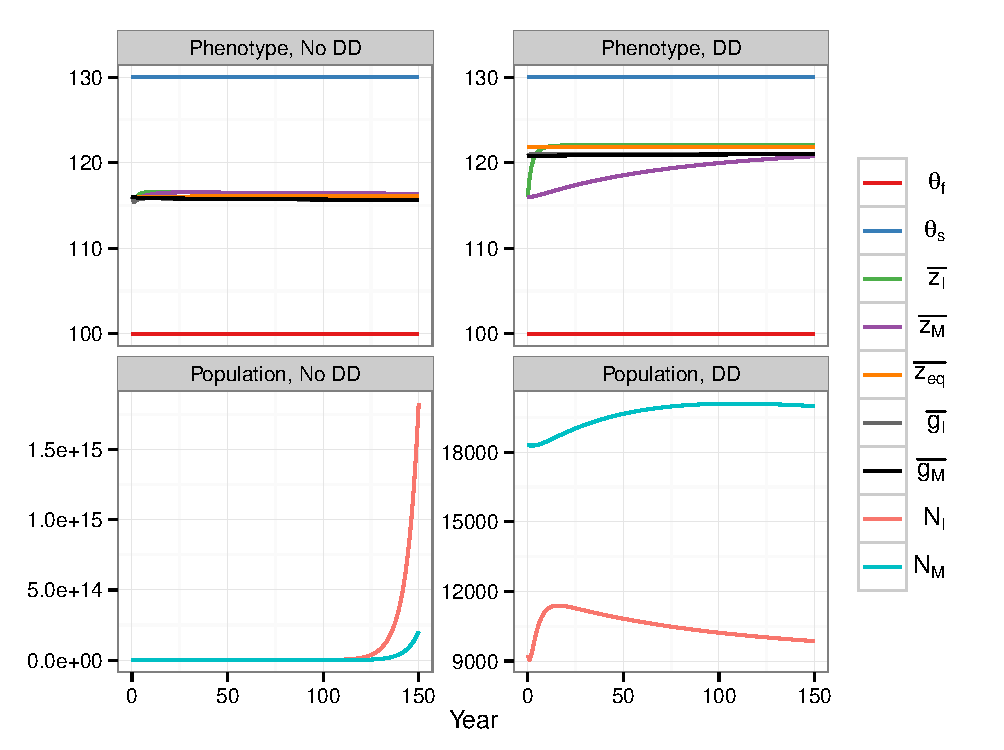
\includegraphics[scale=1]{Figures/DDphenopop.pdf}
	\caption{\textbf{Effect of density-dependence on phenotypes and populations}. \textbf{Top}: Phenotype variations in population ($\overline{z_I}, \overline{z_M}$, starting from $z = 116$) with their corresponding genotypic values ($\overline{g_I}, \overline{g_M}$), and the approximation given by \autoref{eq:zweak}; \textbf{Bottom}: Population, number of immature individuals ($N_I$, red), number of mature individuals ($N_M$, blue). Starting from Stable-Stage Distribution (SSD) in constant environment. \textbf{No DD} means we used the model without density-dependence, \textbf{DD} means we implemented density-dependence through $s_0$ (see \autoref{eq:ddfunc}). Here, bud-burst date is expressed in julian days (numbered days in the year, 1st of January being 1 in julian days).}
	\label{fig:dd}
\end{figure}

\begin{figure}[ht!]
	\centering
	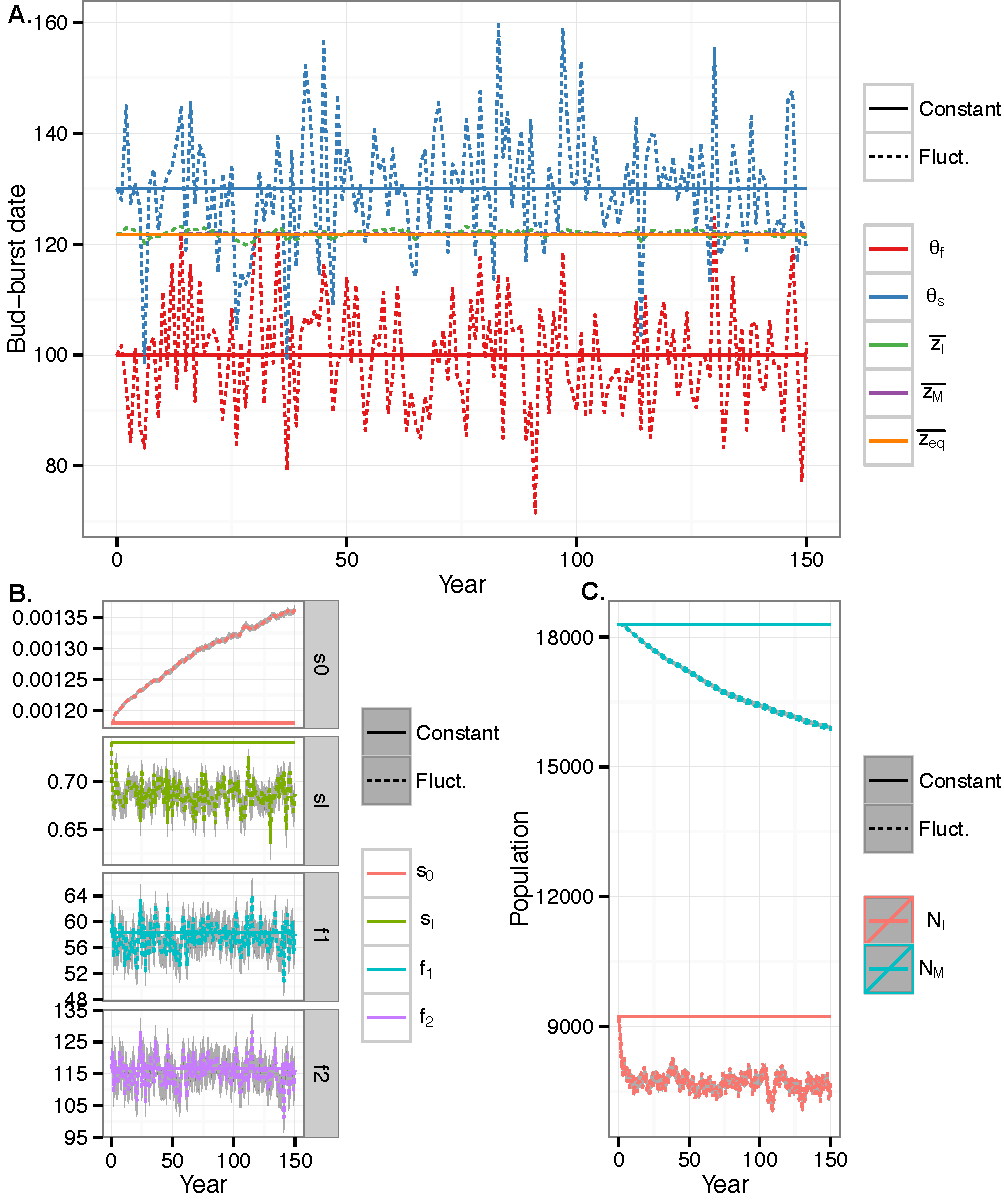
\includegraphics[scale=1]{Figures/PhenoLHTwithCorr.pdf}
	\caption{\textbf{Fluctuating optima against constant environment}. \textbf{Top:} comparison of phenotypes from simulations with constant or fluctuating optima, $\overline{z_{eq}}$ is the approximation shown in \autoref{eq:zweak} results from single simulation. \textbf{Bottom:} (\textbf{Left}) life-history traits in constant or fluctuating environment, (\textbf{Right}) population in constant or fluctuating environment, $N_I$ is the number of immature individuals and $N_M$ the number of mature individuals, population started from the stable stage distribution. \textbf{Solid lines:} values in constant environment, \textbf{Dashed lines:} in fluctuating environment, results were averaged over 100 independent simulations.}
	\label{fig:corr}
\end{figure}

\begin{figure}[ht!]
	\centering
	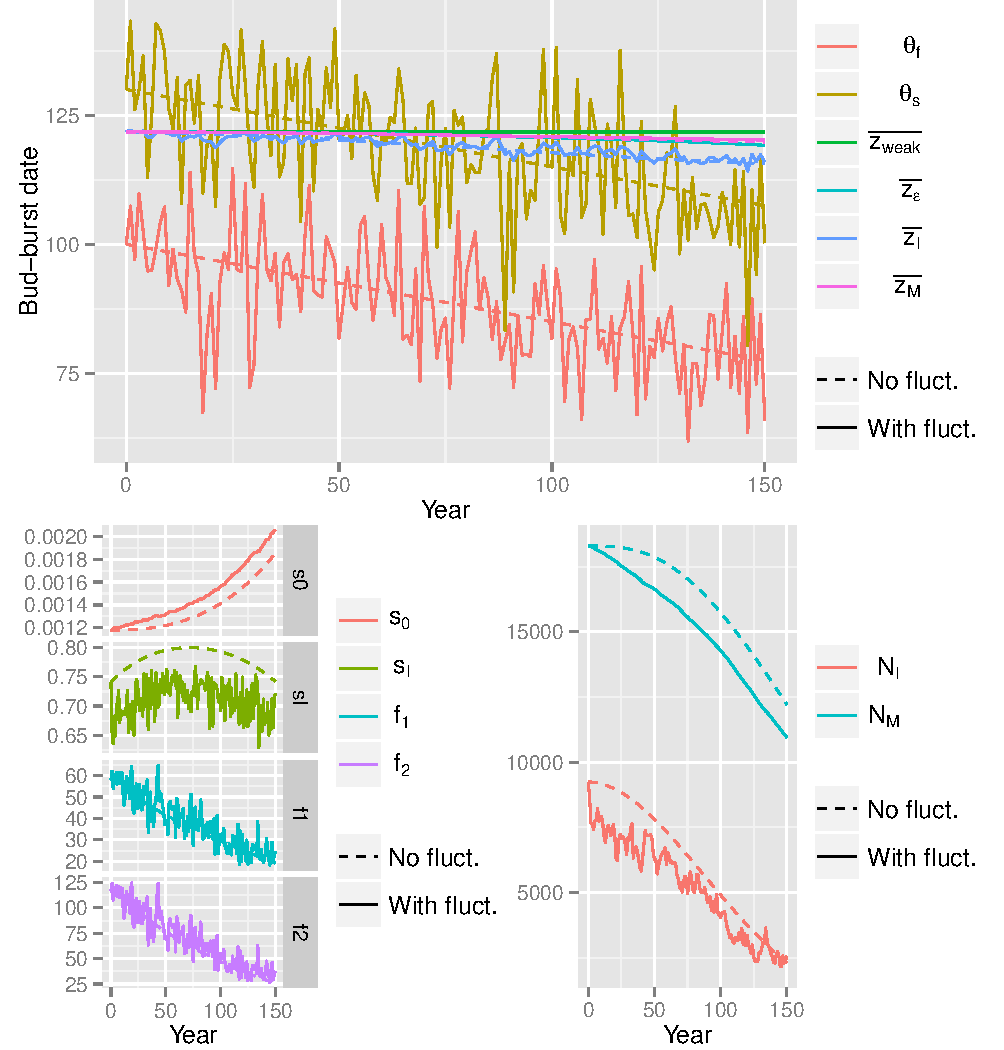
\includegraphics[scale=1]{Figures/Trend.pdf}
	\caption{\textbf{Mixed influences of trend and fluctuations on the population}. \textbf{Top:} Phenotype evolution with and without fluctuations, results from a \textbf{single} simulation; \textbf{Bottom:} (\textbf{Left}) life-history traits evolution; (\textbf{Right}) demography. \textbf{Solid lines:} (\textbf{No fluct.}) linearly decreasing optima with time; \textbf{Dashed lines:} \textbf{With fluct.} fluctuating decreasing optima, results were averaged over 100 independent simulations.}
	\label{fig:trend}
\end{figure}

\begin{figure}[ht!]
	\centering
	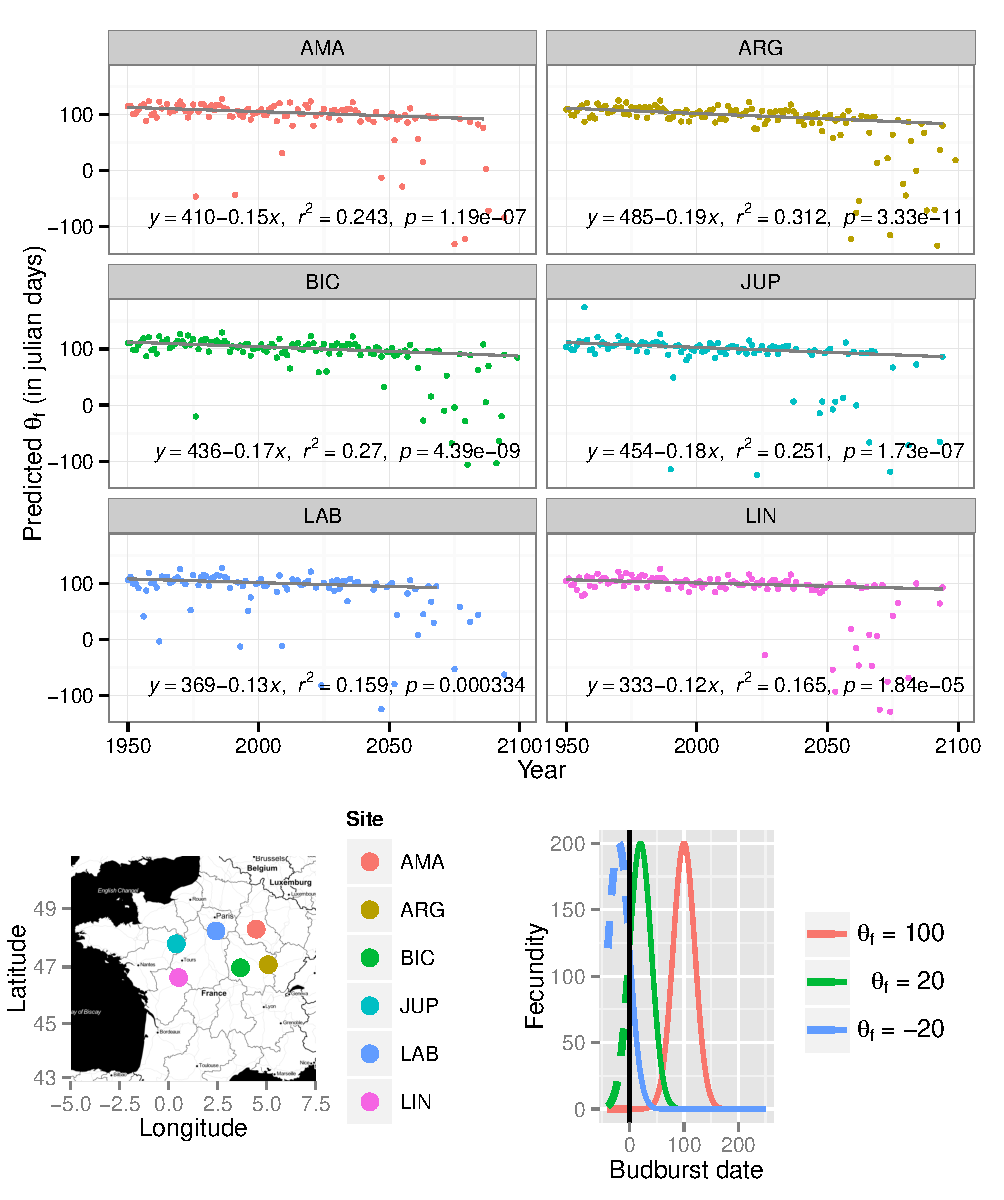
\includegraphics[scale=1]{Figures/optsmaps.pdf}
	\caption{\textbf{$\theta_{f}$ estimations from PHENOFIT data}. \textbf{Top:} estimations of $\theta_f$ for each study site (see \nameref{sec:M&M} for details). \textbf{Bottom:} (\textbf{Left}) map of the study sites; (\textbf{Right}) Theoretical fecundity functions with parameters from~\autoref{tab:params} with values of $\theta_f$ equals to $100$, $20$ and $-20$, solid lines indicate achievable phenotype, dashed lines show theoretical curves but unreachable phenotypes.}
	\label{fig:thetaf}
\end{figure}

\end{document}